% To avoid compiling stuff other than what you're working on right
% now, change the following command giving your file as its
% argument. Also, you have to modify the \input part inside the 
% \begin{document} section
\includeonly{RASD_Main}

% From now on, these are all the packages, colors and variables 
% used by all files
%%%% LAYOUT AND FONTS
\documentclass[12pt]{article}
\DeclareTextFontCommand{\emph}{\bfseries\em}

%%%% PACKAGES
\usepackage[utf8]{inputenc}
\usepackage{color}
\usepackage{caption}

% Used to specify a new tex language(Alloy)
\usepackage{listings}%
\usepackage{Alloy_mine}

\usepackage{graphicx}
\graphicspath{ {../Diagrams/} }

% To split tables b/w pages
\usepackage{longtable}
\usepackage{enumitem}

%\usepackage[shortlabels]{enumerate}

%%%% GLOBAL VARIABLES
\setcounter{secnumdepth}{4}
%S: TOC Depth set to 3 as specified by Prof during lessons
\setcounter{tocdepth}{3}


%%%% COLORS
\definecolor{numbersRed}{RGB}{255, 0, 0}
\definecolor{eclipseBlue}{RGB}{42,0.0,255}
\definecolor{eclipseGreen}{RGB}{63,127,95}
\definecolor{eclipsePurple}{RGB}{127,0,85}

%%%% Actual document, remember to modify the \input part to
%%%% include your file
\begin{document}
\title{Requirement Analysis and Specification Document for PowerEnJoy}
\author{Enrico Migliorini, Alessandro Paglialonga, Simone Perriello}
\clearpage
\maketitle
\clearpage
\tableofcontents

\clearpage
\subsection{Purpose}
This paper represents the \textbf{R}equirement \textbf{A}nalysis and \textbf{S}pecification \textbf{D}ocument of the \textit{System} under development, which will implement the \emph{PowerEnJoy Car-Sharing} Service. This document aims at explaining the functionalities of the System in terms of Functional Requirements, NonFunctional Requirements and Special Requirements, represented using both diagrams and natural language.

The above is a comprehensive list of functionalities provided by the System, that actually translates into a list of goals that the system should reach.

\begin{enumerate}[label=\textbf{G\arabic*}]
	\item The System should allow the registration of the Visitors with their credentials and payment informations.
	\item The System should be able to give each User the list of all the available cars in a range of 5 km from their GPS position or a specific address.
	\item The System should allow each of its Users to reserve a Car whose state is Available.
	\item The System should allow each User to unlock a previously reserved Car when they are in a distance range of 15 meters from the same Car.
	\item If an User has reserved a Car and they did not unlock it within 1 hour from the reservation, the reservation expires, the System sets the Car state as Available again, and the User pays a fixed Fee of 1 EUR.  
	\item The System should allow Users to drive a Car which they have previously unlocked.
	\item The System should be able to know the time usage of the Car, measured in minutes and rounded up.
	\item The System should allow Users to know where are located the Parking and Charging Areas.
	\item The System should allow each User to end the ride in a Parking or Charging Area.
	\item If the System detects the User took at least two other passengers onto the Car for at least 3 minutes, the system applies a discount of 10\% on the last ride.
	\item If a Car is left with no more than 50\% of the battery empty, the System applies a discount of 20\% on the last ride. 
	\item If a Car is left in a Charging Area and the User takes care of plugging the Car into a Socket, the System applies a discount of 30\% on the last ride.
	\item If a Car is left at more than 3 KM from the nearest Charging Area or with more than 80\% of the Battery empty, the system charges 30\% more on the last ride to compensate for the cost required to recharge the car on-site.
	\item If the User enables the money saving option, he/she can input his/her final destination and the System provides the address of the Charging Area where to leave the Car in order to get a Discount on the total Fee. The Charging Area is determined by the System to ensure a uniform distribution of Cars in the city and depends both on the destination of the User and on the availability of Sockets at the selected Charging Area.
\end{enumerate}

\subsection{Intended Audience}
This document is addressed to all the stakeholders involved in the \emph{PowerEnJoy} project. This includes, but it is not limited to, the development committee, product designers and engineers, quality assurance, who will decide if the requirements described in this document have met the intended system requirements.

\subsection{Product Scope}
The aim of the \emph{PowerEnJoy} project is to provide a \textit{Car-Sharing} Service which implements electric-powered cars only.
This system will have to interface the Cars, Charging Areas, allowing Users to reserve, unlock, drive and park Cars, finally charging them the cost of the ride. 
The System will keep track of Cars' position, battery level, possible damages, plugging state.

An useful approach we have used in this phase is based on the distinction between world and machine requirements, as proposed by M. Jackson and P. Zave.

In this approach, the machine represents the system to be developed, while the world is the environment in which the machine operates.
The System under development will define the machine, but has no influence on the world.

There is also a shared set of phenomena that specify, at a high level, the requirements of our System.

The analysis led to the image represented in Figure \ref{fig:WorldMachine}.
%TODO Add sth here
\begin{figure}[!htbp]
\centering
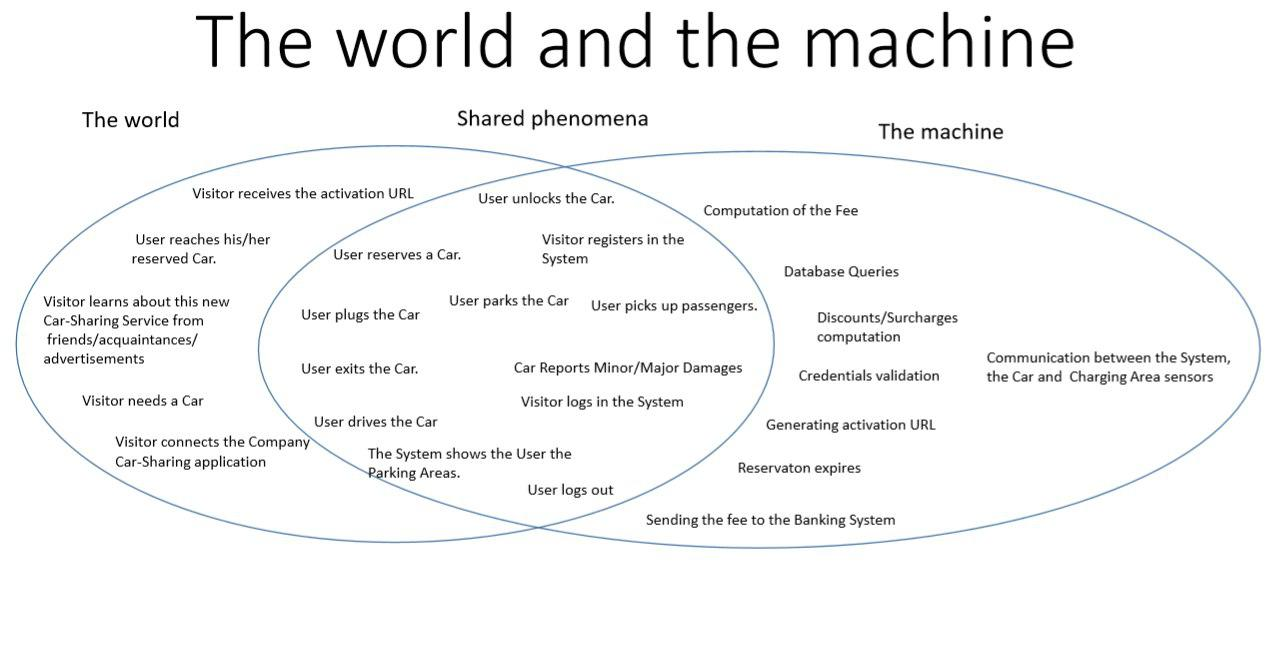
\includegraphics[width=\linewidth,keepaspectratio]{../The_world_and_the_machine.jpg}
\caption{The World And The Machine}
\end{figure}
\label{fig:WorldMachine}
\FloatBarrier

\subsection{Definitions, Acronyms and Abbreviations}
\subsubsection{Business terms glossary}
\paragraph{User related terms}
\begin{itemize}
	\item \emph{Account} \\
	An Account is a virtual representation of a User in the System and contains all the User information relevant to the System. To note that an Account can be either Active or Inactive depending on various condition. For example, an User making a registration to the System is Inactive until he clicks on the activation link sent by the Mailing System. Also, the Company can decide to make an Account Inactive for reasons beyond the scope of this System.
	Moreover, in this System there is no distinction between normal and privileged accounts, id est there are no special roles defined for particular Users. All the maintenance operations are done directly on the Database.
	External operations required by the Company (e.g. an Employee wants to set a machine as Unavailable after a Minor Damage) are done directly by the Company, directly modifying specific part of the Database.
	
	\item \emph{Device}
	It is the piece of hardware used by the User to run the Application. There is no strict requirements on the kind of device an User can have, except that to use most of the System functionalities it should have a working GPS module.
			
	\item \emph{User}\\
	A person registered on the System and that have an associated Account. To note that the terms Account and User are often used interchangeably in this document.

	\item \emph{Visitor}\\
	A person who needs to register or log in to use the System functionalities.	
	\end{itemize}
	
\paragraph{Car related terms}
\begin{itemize}
	\item \emph{Battery} \\
	A Battery powers a Vehicle. The charge state of the Battery can be anywhere between 0\% and 100\%, is reduced when the Vehicle is In Use, and increases when the Vehicle is Plugged to a Charging Area.
		
	\item \emph{Car} \\
	An electric car owned by the Car-sharing service, rented to the User and tracked by the System. A Car can be in one of the following states:
	\begin{itemize}
		\item \textit{In Use}, if it has been unlocked. In this state, it cannot be Reserved by an User.
		\item \textit{Available}, if it can be Reserved by an User.
		\item \textit{Reserved}, if an User has reserved it but has still not unlocked it.
		\item \textit{Unavailable} if it can't be \textit{Reserved} by any User (for example due to damage, battery exhaustion, maintenance, ...)
	\end{itemize}
	Additionally, the \textit{Plugged} flag indicates if the {Car} is plugged or not to a socket of a Charging Area.
	Each Car has a set of sensors used to communicate to the System its position, the status of its battery, its damages, the connection to an electrical socket and the number of seats occupied. It also has a display to show various information to the User. In the end, among the actuators, it is worth mentioning those in charge of the remote unlock of the Car.
	
	\item \emph{Car Board} \\
	It is a piece of hardware and software that has to be installed on each Car to enable the communication between the Car and the Backend. It is responsible to fetch the data of the sensors installed on the Car and to send the Current Fee to the Car display. It is part of the System under development.
				
	\item \emph{Damage} \\
	The Car are able to detect damages, including their entity. In case of damage, the PowerEnjoy board will notify the System. 
	A Car can detect two kind of damages:
	\begin{itemize}
		\item \textit{Major}, a serious damage that prevent the normal usage of the Car (e.g. a damage of a mechanical component). Note that in this case the Car will immediately notify the System and the Car will be set as Unavailable.
		\item \textit{Minor}, a damage that do not prevent the normal usage of the Car (e.g. a scratch or a dent on the car body). Note that in this case, if the Damage is detected during a Ride, the Car will be set as Unavailable only at the end of the Ride.
	\end{itemize}
	In both cases the System will also communicate the damage to the Company. It is up to the Company the decision on how to proceed, but it is meaningful to note that there is no mechanism that will revert the state of the Car as Available, so the suggestion is to dispatch an Employee to the Car in order to evaluate the damages and the best action to take (for example to immediately set the Car as Available again).
	
	\item \emph{Passenger}\\
	Any person who travels in a Car, including the driver. 
	
	\item \emph{Plug}\\
	A part of the Car that can be inserted in a Socket of a Charging Area.
	
	\item \emph{Reservation}\\
	A User performs a Reservation in order to book an Available Car. There are two main constraints on a Reservation: 1) an User can only have one active Reservation at a time and 2) a Reservation expires after a given amount of time (one hour), at the end of which the User will be charged with a Fee of 1E.

	\item \emph{Ride}\\
	Represents the travel done with the Car by the User. It starts from the moment the User ignites the engine of the Car and ends when the Car is parked in a Parking Area,the User and all the other passengers exit the Car.		
\end{itemize}
	
\paragraph{Area related terms}
\begin{itemize}
	\item \emph{Charging Area} \\		
	A special Parking Area where Cars plugs can be connected to the socket in order to recharge their Battery.	
	
	\item \emph{Parking Area}\\
	A place where the User can leave their Car and exit it to end the Ride. Parking Areas are predefined by the System.
	
	\item \emph{Socket}\\
	A part of the Charging Area that can be connected with the Plug of a Car. 
\end{itemize}

\paragraph{Banking related terms}
\begin{itemize}
	\item \emph{Current Fee}\\
	This fee is related to a Ride and is evaluated as 
		
	$\textit{Time usage of the Car} \cdot \textit{Fee per minute}$ 
		
	where \textit{Time usage of the Car} is the time interval between the start and the end of the ride (rounded up to minutes) and \textit{Fee per minute} indicates the rate decided by the Company for every minute of ride.
		
	\item \emph{Discount} \\
	A reduction in the Fee because of good behaviour on the part of the User, e.g. leaving the Cars plugged or bringing it back with a mostly-full battery. The actions that constitute good behaviour are determined ad detailed further in the document.
	
	\item \emph{Fee}\\
	The final amount of money that the Users will be charged for their usage of the Car-sharing service, or for making a Reservation that is not fulfilled.
			
	\item \emph{Surcharge}\\
	An increase in the Fee caused by an improper behaviour on the part of the User, e.g. bringing the Cars back with a mostly-empty battery.
\end{itemize}

\paragraph{External systems}
\begin{itemize}
	\item \emph{Banking System}
	An external system that allows the System to charge the users for a Fee.
		
	\item \emph{Mailing System}
	An external system that allows to send emails to Visitors and Users.
	
	\item \emph{Mapping System}
	An external system that is designed to capture, store, manipulate, analyze, manage, and present spatial or geographical data. 
	It is used in particular to show the GPS position of Cars, Users and Parking Areas on a map, check for existing addresses and get the exact desired position in a specified address.
	
	\item \emph{GPS module}
	A module pre-installed onto User Devices and Cars used to get GPS information.
\end{itemize}
	
\paragraph{System terms}
\begin{itemize}
	\item \emph{Application} \\
	It is the part of the System which acts as a graphical interface between the User and the Backend and allows the User to access the System functionalities.

	\item \emph{Backend}\\
	It is the part of the System which collects input from users for processing.
		
	\item \emph{Database} \label{var:database}\\
	A structure that holds all the information used by the System. For instance, a Database could hold records of every User, Car, every time a User rented a Car and so on. 
	The Company will have the privileges to read all data into our Database at any time. It will also have the ability to write or modify specific portion of data such as:
	\begin{itemize}
		\item set a specific Car as Available/Unavailable;
		\item add a new Car together with its plate number;
		\item set a specific User as Active/Inactive;
		\item mark a Damage as solved, adding additional information to a pre-existing Damage;
		\item mark a specific banking transaction as paid;
		\item creating new Parking or Charging Area together with its internal identifier;
		\item modifying pre-existing Parking and Charging Area informations (such as GPS coordinates, city, internal id, parking and/or charging slots).
	\end{itemize}
	
	\item \emph{Developer}
	Every person concerned with facets of the software development process of this System, including the research, design, programming, and testing. 
	
	\item \emph{System}\\
	The software structure this document is about. At a very high level, it is composed by the Application, the Backend, the Database and the Car Board.
\end{itemize}

\paragraph{Other terms}
\begin{itemize}
	\item \emph{Car-sharing} \\
	A Car-sharing service allows Users to rent Cars for a limited amount of time, being charged a Fee according to time and possibly applying a Discount or a Surcharge.	
	
	\item \emph{Company} \\
	The enterprise that wants to build the System to provide a \textit{Car-Sharing} Service. It represents the main stakeholder.		
		
	\item \emph{Employee}\\
	Any person paid by the Company which should interact with the Power Enjoy System and is not a Developer.
	An Employee, for example, is in charge of every kind of Car maintenance (e.g. charging the Car battery on-site, moving a Car to a Charging Area, detect and quantify damages on a Car, ...). 
	An Employee has also access to specific part of the Database in order to fullfil his/her tasks (see \ref{var:database} - Database).
	The employees and their tasks are managed directed by the Company and this System does not offer any functionality used to help their management.
	
	\item \emph{GPS}\\
	Global Positioning System, it is widely used by the Application to get Users GPS position and by the Car Board to get Car GPS position. The GPS position of Areas, on the other hand, is predefined and will be retrieved directly from the \emph{Database}.
\end{itemize}

\subsubsection{Document specific terms}
\begin{itemize}
	\item \emph{Alloy} 
	A descriptive language that allows to describe a set of structures through constraints.
	
	\item \emph{Internet Protocol Suite}
	The set of communications protocols used on the Internet. It is commonly known as \textbf{TCP/IP}.
	
	\item \emph{HTTP(S)}
	One of the application protocols of the Internet Protocol Suite, widely used by our System.
	
	\item \emph{RASD}
	Requirements Analysis and Specification Document. This document, describing the \emph{System} to be developed.
	
	\item \emph{UC}
	Use Case. A description of interaction between \emph{User}s and \emph{System}.
	
	\item \emph{UML}
	Unified Modeling Language. A language for modeling Object-Oriented software systems.
\end{itemize}

\clearpage
This section will give a broad overview of the whole System under development. It will explain how the System interacts with external systems and introduce its main functionality.

It will also describe the end users and the functionalities of the System reserved to them, detailing all the informations relevant to clarify their needs.

At last it will present the constraints and assumptions made for the System under development.

\subsection{Product Perspective}

This System will be implemented ex-novo to support all the functionalities required by the \textit{PowerEnJoy Car-Sharing} Service.

The System will be able to communicate with all the involved external systems, such as the Database,in which all the information are stored and can be modified by the System, the Banking System, needed to perform the monetary transactions, the Mailing System, which will forward the emails generated by the System, and the Mapping System, which is used in particular to show the GPS position of Cars, Users and Parking Areas on a map, check for existing addresses, and get the exact desired position in a specified address. The System will adopt the HTTP(S) protocol to communicate with the above specified systems managing the interactions through a set of shared protocols and APIs.
\smallskip

End users will access the System functionalities through an Internet connection, using the User intended interface of the System, the Application. Hence, the System should also be able to implement the Application Layer of the Internet Protocol Suite.
Users will communicate their position to the System using the GPS coordinates in order to unlock the previously reserved Car.
\smallskip

At last, the System should be able to communicate with the wide variety of sensors placed inside the Cars, in order to know, in every moment, their position, the status of their battery, their possible damages, their plugged status and the number of seats occupied. 

\subsubsection{Class Diagram}
%TODO...
\subsubsection{Statechart}
%TODO...


\subsection{Product Functions}
Using the the Application, the User will be able to register an account in the System, log in the System and so finally access the System functionalities dedicated to users. The User can now locate all the Cars, whose state is \textit{Available}, specifying a desired address or asking the System to locate him/her through the GPS coordinates.\\
The Mapping System is now asked to check for the existence of the specified address or locate the User's position, showing on the map all the \textit{Available} Cars, together with their intrinsic information, in a distance range specified by the System. 
\smallskip

The User can now decide to reserve a Car, from this moment a one hour countdown starts during which the User will be able to unlock his/her reserved Car.
The User can unlock the Car asking the System to locate him/her and if the Mapping System verifies that the User is in a specified distance range from the Car, the Car is unlocked and the User can now enter and drive it. If the User doesn't unlock the Car during the previous specified time period, the System cancels the reservation, sets the Car status as \textit{Available} and communicates to the Banking System the application of a fee.
\smallskip


At the end of the ride, the System, basing on the time usage period of the Car, and on bad or good behaviors preset by the System will evaluate the Fee and notify and the Banking System of the total amount to charge to the User's credit card.


%TODO format requirements
\newcounter{RequirementsCounter}
\stepcounter{RequirementsCounter}

%\begin{center}
%  \begin{longtable}{|p{.2\textwidth}|p{.12\textwidth}|p{.58\textwidth}|}
%    \hline
%    \textbf{Goal} & \textbf{Priority} & \textbf{Function} \\ \hline
%    Registration & High & Allows a Visitor to register their credentials, becoming a User \\ \hline
%    Login & High & Lets a User access the system \\ \hline
%    Find Nearby Cars & ? & Shows Available Cars in a location \\ \hline
%    Reservation & ? & Allows a user to set a nearby Car as Reserved \\ \hline
%    Proximity Unlock & ? & Unlocks the car when the User who Reserved it is close \\ \hline
%  \end{longtable}
%\end{center}

\subsection{User Classes and Characteristics}
\begin{center}
  \begin{tabular}{|p{.2\textwidth}|p{.39\textwidth}|p{.39\textwidth}|}
    \hline
    \textbf{Name} & \textbf{Description} & \textbf{Actions} \\ \hline
    Visitor & A person who would like to register an account to access the System functionalities. & Can perform the registration and activation of the account. Successively he can log in the System becoming a User.\\\hline
    User & Someone who is registered in the System and can access its functionalities & Can locate, reserve and drive Cars. Will be charged for the use of the Cars. \\ \hline
    \end{tabular}
\end{center}
\vspace{5mm}
External access to the Database provided to Employees and Administrators is under the responsibility and the regulations of the Company and is not managed by this System.


\subsection{Constraints}
\subsubsection{Hardware Constraints}\label{OE}
The device used by the User should be able to establish an internet connection to the System using the Application. In addition, in order to perform the localization, reservation and unlocking of a Car the device must have installed a working GPS module. 

\subsubsection{Design and Implementation Constraints}
The system will employ the HTTP(S) protocol in order to communicate with the Database, the external systems, and with the User through the Application. 

\subsection{Assumptions and Dependencies}
\begin{enumerate}
	\item The User can only have one Account at time.
	\item The Company can decide at any time to block an User from accessing to the System (f.e. for improper behavior, unpaid bill, ...). It will be done by employees or Administrators.
	\item The User always provides real correct data in his/her registration form.
	\item The Database in which the Cars, Parking Areas, Charging Areas, Users,etc, are stored, is owned and managed from the Company (and not by this System), which is responsible for its security, reliability and availability. Our System is provided by the Company with read/write access to this Database.
	\item The Company is responsible for the employees and their actions.
	\item The Car has a set of sensors that can detect, in every moment, its position, the status of its battery, the status of the engine, its damages, the connection of its plug to an electrical socket and the number of seats occupied. We assume that these sensors won't ever break down and that their measures are always correct.
	\item The Car GPS always detects its position with absolute precision.
	\item The User always enters the Car when he/she unlocks its doors.	
	\item After a Car is Plugged, it will not be maliciously unplugged by the User himself/herself or by other people.
	\item After the doors of the cars are unlocked by the User, he/she always enters the Car, ignites the engine and leave the Parking Area.
	\item An User can park/stop the Car everywhere and leave the Car at anytime. However, the system will end the ride (i.e. stop charging the User) only if he/she turns the engine off inside a Parking Area.
	\item When the User gets at least two Passengers, the corresponding discount on the User's fee will be applied only if the passengers stay together in the Car for more than 3 minutes. 
	\item When a User will park the Car inside a Parking Area, it will always correctly use one and only one free slot.
	\item As soon as the Car battery status gets below 20\% of the full capacity AND the Car isn't in a Charging Area AND the Car Status isn't \textit{In Use} OR \textit{Plugged}, there's always an Employee that immediately reaches the Car and recharges it on site; in the meanwhile the Car status is \textit{Unavailable}.	
	\item When the Car is \textit{In Use} and the battery charge level reaches the 0\% of the full capacity the Car stops working and is immediately set as \textit{Unavailable}.
	If the Car status is \textit{Unavailable}, the Car will be reached by an Employee to consider if the Car needs to be taken in the Company's workshop for repairs or just needs to be recharged.
	\item The Car has the ability to detect if it has been damaged. 
	\item If the Car status is \textit{In Use} when a \textit{Minor damage} is detected, the Car status will be set to \textit{Unavailable} at the end of the ride; if a \textit{Major damage} is detected the Car status is immediately set to \textit{Unavailable}. In both cases an employee will reach the car and cope with the damages, deciding if the Car can be immediately used again (sets it to \textit{Available}) or should be moved to the Company's workshop and/or if the User should pay for the damages. 
	\item A car which is \textit{Available} or \textit{Plugged} can be set as \textit{Unavailable} in every moment by an Employee. This is done through another Company's System as it is not provided in this System.
	\item A car which is \textit{Unavailable} can be set to \textit{Available} in every moment by an Employee.  This is done through another Company's System and it is not provided in this System.
	\item If the Car has been left out of a Parking Area there will always be an employee which immediately reaches it, recharges it and move it to a Charging Area. 
	\item Every fine received by the Company for improper use of the Car will be managed by the Company.
	
\end{enumerate}

\clearpage

\clearpage
\section{Specific Requirements}
\subsection{Functional Requirements}
The functionality for the various users.
\subsubsection {Requirements List}
\begin{enumerate}[label=\textbf{R\arabic*}]
\item PowerEnjoy shall provide Users with the ability to access all the System functionalities reserved to them.
\item PowerEnjoy shall support Users in locating Available Cars within a range of 5 Km from a specific position.
\item PowerEnjoy shall support Users in locating Parking Areas and their free parking slots.
\item PowerEnjoy shall support Users in locating Charging Areas and their free parking slots and free charging sockets.
\item PowerEnjoy shall support Users in reserve Available Cars.
\item PowerEnjoy shall apply a fixed Surcharge of 1 EUR if he/she has reserved a Car and not unlocked it within a time range of 60 minutes.
\item PowerEnjoy shall support a User in unlock a Car he/she has previously reserved when he/she is in a range of 15 meters from the same Car.
\item PowerEnjoy shall charge the User of a fixed fee per minutes, communicating to him/her the Fee he will get charged at the end of the ride basing only on the driving time and the fee per minutes.
\item PowerEnjoy shall be able to know if a User has took in the Car he/she is driving at least two other passengers for at least 3 minutes. If so, PowerEnjoy should apply a percentage Discount of 10\% on the final Fee of the last ride.
\item PowerEnjoy shall allow the User to end the ride in a Parking or Charging Area. 
\item PowerEnjoy shall allow any User who has ended a ride to plug the Car he/she has driven to a Socket in a time rage of 2 minutes since he/she has ended the ride, in order to get a percentage Discount of 30\% on the final Fee of the last ride.
\item PowerEnjoy shall apply a percentage Discount of 20\% on the final Fee of the last ride if the User will end the ride leaving the Car with more than 50\% battery charge status.
\item PowerEnjoy shall apply a percentage Surcharge of 30\% on the final Fee of the last ride if a User leaves the Car at more than 3 km from the nearest Charging Area or with a battery charge status less than 20\%.
\item PowerEnjoy shall provide a User the ability to use the "Money Saving Option", telling him/her the position of a Charging Area where he/she has to park the Car he/she is driving in order to get a Discount on the total Fee. The Charging Area is determined by the System to ensure a uniform distribution of Cars in the city of that address and depends both on the destination of the User and on the availability of Sockets at the selected Charging Area.
\item PowerEnjoy shall interface with an external Mailing System to send emails to Users.
\item PowerEnjoy shall interface with an external Banking System to charge Fee to Users.
\item PowerEnjoy shall interface with an external GPS System to know the positions of Users and Areas.
\item PowerEnjoy shall interface with an external Mapping System to know the positions of Users and Areas.
\item PowerEnjoy shall interface with the existing Car to get their GPS position, damages, connection to an electrical socket, the number of seats occupied. 
\end{enumerate}

\subsubsection{Use cases specification}
% Counter to use for UseCaseId
\newcounter{UseCaseIdCounter}

% It starts from 0 by default, so I've incremented it.
\stepcounter{UseCaseIdCounter}

\begin{longtable}{|p{0.2\linewidth} p{0.8\linewidth}|}
	% Some table settings
	\captionsetup{labelformat=empty} % To not show Table 1, Table 2 under the table
	\caption{\textbf{Register Account}} % Table caption
	\label{UC_Register}%If later on you want to refer to this label, you can this label. 
	\\ \hline % end of row + new horizontal line
	
	% The table itself
	\textbf{ID} & UC\theUseCaseIdCounter \\ \hline
	\textbf{Description} & The \emph{Visitor} wants to create an \emph{Account} for the \emph{Car-Sharing} Service. \\ \hline
	\textbf{Actors} & \emph{Visitor}.\\ \hline
	\textbf{Pre-Conditions} & The \emph{Visitor} connects to the \emph{Company's Car-Sharing}WebSite/Application. \\ \hline
	\textbf{Flow of events} & 
		\begin{enumerate}
			\item The \emph{Visitor} selects the function \textit{\textquotedblleft{Sign Up}\textquotedblright}.
			\item The \emph{System} returns a form to enter all the required data: Name, Surname, Birth date, ID Card Number, Driving License number and Credit Card number. It also asks for an email address and a password which will be used for the future logins.
			\item The \emph{Visitor} fills the form with all the required information.
			\item The \emph{System} stores the request together with all the data provided with it, generates a random activation URL and asks the \emph{Mail System} to forward his/her URL to the email address of the \emph{Visitor}.
		\end{enumerate}	 \\ \hline
	\textbf{Post Conditions} & The \emph{Mail System} sends the activation URL to the \emph{Visitor}'s email provided in the registration form. \\ \hline
	\textbf{Exceptions} & 
		\begin{itemize}
		\item The \emph{System} recognizes invalid or missing data in the form compiled by the emph{Visitor}and informs him/her of the error. The flow of events restarts from point 1.
		\item The Visitor inserts in the form a Social Security Number, or ID Card Number, or Driving License number, or Email Address, which is already present in the System. The System shows an error message saying that some of those credentials were already been inserted into the System for another account. The flow of events restarts from point 1.
		\end{itemize} \\ \hline
\end{longtable}


\stepcounter{UseCaseIdCounter}
\begin{longtable}{|p{0.2\linewidth} p{0.8\linewidth}|}
	% Some table settings
	\captionsetup{labelformat=empty} % To not show Table 1, Table 2 under the table
	\caption{\textbf{Activate Account}} % Table caption
	\label{UC_Activate}	\\ \hline
	
	% The table itself
	\textbf{ID} & UC\theUseCaseIdCounter \\ \hline
	\textbf{Description} & The \emph{Visitor} wants to activate his/her \emph{Account}. \\ \hline
	\textbf{Actors} & \emph{Visitor}.\\ \hline
	\textbf{Pre-Conditions} & The \emph{Visitor} has received the activation URL on his/her mail box. \\ \hline
	\textbf{Flow of ev-ents} & 
	\begin{enumerate}
		\item The \emph{Visitor} opens the received activation URL.
		\item The \emph{System} acknowledges that the Visitor has arrived in his/her activation Web Page and activates his/her account.
	\end{enumerate}	 \\ \hline
	\textbf{Post Conditions} & The \emph{Visitor} is now become an \emph{User} which can access the \emph{System} using the credentials (Email, password) he provided during the registration phase. \\ \hline
	\textbf{Exceptions} & 
	\begin{itemize}
		\item The Activation URL expires after 10 days it has been generated. The Visitor?s data are cancelled from the System and the Visitor will have to perform the Registration (UC1) again.
	\end{itemize} \\ \hline
\end{longtable}

\stepcounter{UseCaseIdCounter}

\begin{longtable}{|p{0.2\linewidth} p{0.8\linewidth}|}
	% Some table settings
	\captionsetup{labelformat=empty} % To not show Table 1, Table 2 under the table
	\caption{\textbf{Log In}} % Table caption
	\label{UC_Login}%If later on you want to refer to this label, you can use this label. 
	\\ \hline % end of row + new horizontal line
	
	% The table itself
	\textbf{ID} & UC\theUseCaseIdCounter \\ \hline
	\textbf{Description} & The \emph{Visitor} wants to log in the \emph{System}. \\ \hline
	\textbf{Actors} & \emph{Visitor}.\\ \hline
	\textbf{Pre-Conditions} & The \emph{Visitor} connects to the Company's \emph{Car-Sharing WebSite/Application} \\ \hline
	\textbf{Flow of events} & 
	\begin{enumerate}
		\item The \emph{Visitor} selects the function \textit{\textquotedblleft{Login}\textquotedblright} .
		\item The \emph{System} shows the \emph{Visitor} a login form, asking him to insert the email and password provided in the registration form.
		\item The \emph{Visitor} inserts the pair (Email,Password) used during the registration phase and selects the function \textit{\textquotedblleft{Log me in}\textquotedblright}
	\end{enumerate}	 \\ \hline
	\textbf{Post Conditions} & The \emph{System} verifies the existence of an account associated with that pair (Email,password) and logs the \emph{Visitor} in. The \emph{Visitor} has now become \emph{User}  \\ \hline
	\textbf{Exceptions} & 
	\begin{itemize}
		\item The Activation URL expires after 10 days it has been generated. The Visitor?s data are cancelled from the System and the Visitor will have to perform the Registration (UC1) again.
	\end{itemize} \\ \hline
\end{longtable}
\stepcounter{UseCaseIdCounter}

\begin{longtable}{|p{0.2\linewidth} p{0.8\linewidth}|}
	% Some table settings
	\captionsetup{labelformat=empty} % To not show Table 1, Table 2 under the table
	\caption{\textbf{Log Out}} % Table caption
	\label{UC_Logout}%If later on you want to refer to this label, you can use this label. 
	\\ \hline % end of row + new horizontal line
	
	% The table itself
	\textbf{ID} & UC\theUseCaseIdCounter \\ \hline
	\textbf{Description} & The User wants to log out from the System. \\ \hline
	\textbf{Actors} & \emph{User}.\\ \hline
	\textbf{Pre-Conditions} & The \emph{User} is logged in the \emph{System} \\ \hline
	\textbf{Flow of events} & 
	\begin{enumerate}
		\item The \emph{User} selects the function \textit{\textquotedblleft{Log out}\textquotedblright} .
		\item The \emph{System} performs the \emph{User}'s logout.
	\end{enumerate}	 \\ \hline
	\textbf{Post Conditions} & The \emph{System} shows the confirmation of the logout to the \emph{User}.
	
	The \emph{User} is now not able to use the \emph{System} functionalities dedicated to Users anymore (until he logs in again). \\ \hline
	\textbf{Exceptions} &  \\
%	\begin{itemize}
%	\end{itemize} \\ 
\hline
\end{longtable}
\stepcounter{UseCaseIdCounter}

\begin{longtable}{|p{0.2\linewidth} p{0.8\linewidth}|}
	% Some table settings
	\captionsetup{labelformat=empty} % To not show Table 1, Table 2 under the table
	\caption{\textbf{Locate Available Cars}} % Table caption
	\label{UC_LocateCars}%If later on you want to refer to this label, you can use this label. 
	\\ \hline % end of row + new horizontal line
	
	% The table itself
	\textbf{ID} & UC\theUseCaseIdCounter \\ \hline
	\textbf{Description} & The \emph{User} wants to locate the avialable \emph{Cars}. \\ \hline
	\textbf{Actors} & \emph{User}.\\ \hline
	\textbf{Pre-Conditions} & The \emph{User} is logged in the \emph{System} \\ \hline
	\textbf{Flow of events} & 
	\begin{enumerate}
		\item The \emph{User} selects the function \textit{\textquotedblleft{Locate Cars}\textquotedblright}.
		\item The \emph{System} shows a text box asking the \emph{User} to provide an address near which they would like to see the \emph{Cars} whose state is \textit{Available}.
		\item The \emph{User} inserts the desired address and selects the \textit{\textquotedblleft{Locate}\textquotedblright} function.
	\end{enumerate}	 \\ \hline
	\textbf{Post Conditions} & The \emph{System} shows the \emph{User} a map containing all the \emph{Cars} whose state is Available and which are within a 5KM range from the provided address. \\ \hline
	\textbf{Alternative Flow of Events} & The \emph{User} selects the function \textit{\textquotedblleft{Near Me}\textquotedblright} instead of inserting a specific address and sends their \emph{GPS Coordinates} to the \emph{System}. \\ \hline
	\textbf{Exceptions} & 
	\begin{itemize}
		\item The System does not find the inserted address and informs the User. The Flow of Events starts from point 1.
		\item There are no available Cars in the specified address/User?s Position. The System informs the User. The Flow of Events start from point 1.
	\end{itemize} \\ \hline
\end{longtable}
\stepcounter{UseCaseIdCounter}

\begin{longtable}{|p{0.2\linewidth} p{0.8\linewidth}|}
	% Some table settings
	\captionsetup{labelformat=empty} % To not show Table 1, Table 2 under the table
	\caption{\textbf{Reserve Available Car}} % Table caption
	\label{UC_ReserveCar}%If later on you want to refer to this label, you can use this label. 
	\\ \hline % end of row + new horizontal line
	
	% The table itself
	\textbf{ID} & UC\theUseCaseIdCounter \\ \hline
	\textbf{Description} & The \emph{User} wants to reserve a \emph{Car}. \\ \hline
	\textbf{Actors} & \emph{User}.\\ \hline
	\textbf{Pre-Conditions} & The \emph{User} is logged in the \emph{System}, the \emph{User} does not have another active reservation, the \emph{User} is not driving another \emph{Car}, and the System has found available \emph{Cars} when the \emph{User} activated the \textit{\textquotedblleft{Locate Available Cars}\textquotedblright} function. \\ \hline
	\textbf{Flow of events} & 
	\begin{enumerate}
		\item The \emph{User} chooses a specific \emph{Car} among those showed on the map.
		\item The \emph{User} selects the function \textit{\textquotedblleft{Reserve this Car}\textquotedblright}.
	\end{enumerate}	 \\ \hline
	\textbf{Post Conditions} & The \emph{System} stores the \emph{Reservation} of the \emph{Car}, changing its status to \emph{Reserved}.
The \emph{System} activates a countdown of 1 hour during which the \emph{User} will have the possibility to unlock the \emph{Reserved} \emph{Car}. \\ \hline
	\textbf{Exceptions} & \\ \hline
\end{longtable}
\stepcounter{UseCaseIdCounter}

\begin{longtable}{|p{0.2\linewidth} p{0.8\linewidth}|}
	% Some table settings
	\captionsetup{labelformat=empty} % To not show Table 1, Table 2 under the table
	\caption{\textbf{Unlock Car}} % Table caption
	\label{UC_UnlockCar}%If later on you want to refer to this label, you can use this label. 
	\\ \hline % end of row + new horizontal line
	
	% The table itself
	\textbf{ID} & UC\theUseCaseIdCounter \\ \hline
	\textbf{Description} & The \emph{User} wants the \emph{System} to open the doors of the \emph{Car} in order to enter it. \\ \hline
	\textbf{Actors} & \emph{User}.\\ \hline
	\textbf{Pre-Conditions} & The \emph{User} is logged in the \emph{System} and has reserved a \emph{Car}. \\ \hline
	\textbf{Flow of events} & 
	\begin{enumerate}
		\item The \emph{User} activates the function\textit{\textquotedblleft{Unlock Car}\textquotedblright}.
		\item The \emph{User} sends their GPS coordinates to the \emph{System}.
		\item The \emph{System} checks that the GPS coordinates of the \emph{User} are within a 15 metres range from those of the \emph{Car} itself.
	\end{enumerate}	 \\ \hline
	\textbf{Post Conditions} & The \emph{System} has verified that the \emph{User} is nearby the car (within the specified distance range) and unlocks the \emph{Car}'s doors.
	 
The \emph{System} then changes the \emph{Car} status to \emph{In Use} and sets the \emph{Plugged} Flag to False.

The \emph{User} enters the \emph{Car}. \\ \hline
	\textbf{Exceptions} & If one hour has passed since the reservation has been made and the \emph{User} hasn't unlocked the Car, either because he wasn't within the 15 meters distance range or didn't activate this function, then:
	\begin{itemize}
	\item The reservation expires, so that the \emph{User} cannot unlock the \emph{Car} anymore (unless they reserve it again).
	\item The \emph{System} changes the \emph{Car}'s status to \emph{Available}.
	\item The \emph{System} communicates to the \emph{Banking System} the \emph{Fee} to charge the \emph{User} (this sum amounts to 1 EUR).
	\item The \emph{System} allows the \emph{User} to perform another reservation.
	\end{itemize} \\ \hline
\end{longtable}
\stepcounter{UseCaseIdCounter}

\begin{longtable}{|p{0.2\linewidth} p{0.8\linewidth}|}
	% Some table settings
	\captionsetup{labelformat=empty} % To not show Table 1, Table 2 under the table
	\caption{\textbf{Drive Car}} % Table caption
	\label{UC_DriveCar}%If later on you want to refer to this label, you can use this label. 
	\\ \hline % end of row + new horizontal line
	
	% The table itself
	\textbf{ID} & UC\theUseCaseIdCounter \\ \hline
	\textbf{Description} & The \emph{User} starts driving the \emph{Reserved} \emph{Car}. \\ \hline
	\textbf{Actors} & \emph{User}.\\ \hline
	\textbf{Pre-Conditions} & The \emph{User} has unlocked the doors of the \emph{Car} and entered it. \\ \hline
	\textbf{Flow of events} & 
	\begin{enumerate}
		\item The \emph{User} starts the engine of the \emph{Car}.
		\item The \emph{System} starts the Ride Timer which indicates the time usage of the \emph{Car}.
		\item {[}Extension Point UC 9{]}
		\item {[}Extension Point UC 12{]}
		\item The \emph{System} calculates the current \emph{Fee} charged to the \emph{User} (calculated as a given amount of money per minute on the Ride Timer) while showing it on the on-board screen.
	\end{enumerate}	 \\ \hline
	\textbf{Post Conditions} & The \emph{User} drives the \emph{Car} \\ \hline
	\textbf{Exceptions} & \\ \hline
\end{longtable}
\stepcounter{UseCaseIdCounter}

\begin{longtable}{|p{0.2\linewidth} p{0.8\linewidth}|}
	% Some table settings
	\captionsetup{labelformat=empty} % To not show Table 1, Table 2 under the table
	\caption{\textbf{Drive With Passengers $<<$extends UC 8$>>$}} % Table caption
	\label{UC_DriveWithPassengers}%If later on you want to refer to this label, you can use this label. 
	\\ \hline % end of row + new horizontal line
	
	% The table itself
	\textbf{ID} & UC\theUseCaseIdCounter \\ \hline
	\textbf{Description} & The \emph{User} picks up \emph{Passengers} to share the ride with. \\ \hline
	\textbf{Actors} & \emph{User}.\\ \hline
	\textbf{Pre-Conditions} & The \emph{User} is driving their \emph{Reserved} \emph{Car}. \\ \hline
	\textbf{Flow of events} & 
	\begin{enumerate}
		\item The \emph{User} picks up the \emph{Passengers}.
		\item The \emph{Car} detects the presence and number of the \emph{Passengers}.
	\end{enumerate}	 \\ \hline
	\textbf{Post Conditions} & The \emph{User} is sharing the ride with their \emph{Passengers}.
	
	The \emph{System} stores the number of \emph{Passengers} who were picked up and whether they stayed in the \emph{Car} for at least 3 minutes.\\ \hline
	\textbf{Exceptions} & \\ \hline
\end{longtable}
\stepcounter{UseCaseIdCounter}

\begin{longtable}{|p{0.2\linewidth} p{0.8\linewidth}|}
	% Some table settings
	\captionsetup{labelformat=empty} % To not show Table 1, Table 2 under the table
	\caption{\textbf{End Ride}} % Table caption
	\label{UC_EndRide}%If later on you want to refer to this label, you can use this label. 
	\\ \hline % end of row + new horizontal line
	
	% The table itself
	\textbf{ID} & UC\theUseCaseIdCounter \\ \hline
	\textbf{Description} & The \emph{User} ends the ride and the \emph{System} processes the \emph{Fee}. \\ \hline
	\textbf{Actors} & \emph{User}.\\ \hline
	\textbf{Pre-Conditions} & The \emph{User} parks the \emph{Car} in one of the \emph{Parking Areas}. \\ \hline
	\textbf{Flow of events} & 
	\begin{enumerate}
		\item The \emph{User} exits the \emph{Car}.
		\item The \emph{System} verifies that no one is in the \emph{Car}.
		\item The \emph{System} checks the \emph{Battery} status. 
		\item The \emph{System} checks, via the GPS coordinates, whether the \emph{User} has left the \emph{Car} within a 3KM distance range from the nearest \emph{Charging Area}.
		\item The \emph{System} checks if the \emph{User} drove with \emph{Passengers} (UC9).
		\item {[}Extension Point UC11{]}.
	\end{enumerate}	 \\ \hline
	\textbf{Post Conditions} & The \emph{System} locks the doors of the \emph{Car} and sets its status to \emph{Available}.
	
	The \emph{System} communicates to the \emph{Banking System} the final \emph{Fee} to charge the \emph{User}. \\ \hline
	\textbf{Alternative Flow of Events} & 
	\begin{itemize}
		\item The \emph{Battery} status is higher than 50\%, the \emph{User} didn't or did take at least 2 \emph{Passengers} with him for at least 3 minutes (UC9), didn't leave the \emph{Car} further than 3KM from the nearest \emph{Charging Area}, didn't plug the \emph{Car} (UC11), hence the System applies a 20\% \emph{Discount} on the \emph{Fee} of the last ride and communicates it to the \emph{Banking System} the \emph{Fee} which will be charged to the \emph{User}.
		\item The \emph{User} did plug the \emph{Car} (UC11), the \emph{Battery} status is higher than or equal to 20\%, they didn't or did take at least 2 \emph{Passengers} with him for at least 3 minutes (UC9), hence the System applies a 30\% \emph{Discount} on the \emph{Fee} of the last ride and communicates to the \emph{Banking System} the \emph{Fee} which will be charged to the \emph{User}.
		\item The \emph{User} did plug the \emph{Car} (UC11), the \emph{Battery} status is lower than 20\%, they didn't or did take at least 2 \emph{Passengers} with him for at least 3 minutes (UC9), hence the System doesn't apply any \emph{Discount} or \emph{Surcharge} on the \emph{Fee} of the last ride and communicates to the \emph{Banking System} the \emph{Fee} which will be charged to the \emph{User}.
		\item The \emph{User} didn't plug the \emph{Car} (UC11), the \emph{Battery} status is higher than 50\%, they either did or didn't take at least 2 \emph{Passengers} with him for at least 3 minutes (UC9), did leave the \emph{Car} further than 3KM from the nearest \emph{Charging Area}, hence the System applies a 10\% \emph{Surcharge} on the \emph{Fee} of the last ride and communicates to the \emph{Banking System} the \emph{Fee} which will be charged to the \emph{User}.
		% Even longtable can't handle tables this long
		\end{itemize} \\ &
		\begin{itemize}
		\item The \emph{Battery} status is between 20\% and 50\% (included), the \emph{User} did take at least 2 \emph{Passengers} with him for at least 3 minutes (UC9), didn't leave the \emph{Car} further than 3KM from the nearest \emph{Charging Area}, didn't plug the \emph{Car} (UC11), hence the System applies a 10\% \emph{Discount} on the \emph{Fee} of the last ride and communicates to the \emph{Banking System} the \emph{Fee} which will be charged to the \emph{User}.
		\item The \emph{Battery} status is lower than 20\%, the \emph{User} did take at least 2 \emph{Passengers} with him for at least 3 minutes (UC9), either did or didn't leave the \emph{Car} further than 3KM from the nearest \emph{Charging Area}, didn't plug the \emph{Car} (UC11), hence the System applies a 20\% \emph{Surcharge} on the \emph{Fee} of the last ride and communicates to the \emph{Banking System} the \emph{Fee} which will be charged to the \emph{User}.
		\item The \emph{Battery} status is between 20\% and 50\% (included), the \emph{User} did take at least 2 \emph{Passengers} with him for at least 3 minutes (UC9), did leave the \emph{Car} further than 3KM from the nearest \emph{Charging Area}, hence the System applies a 20\% \emph{Surcharge} on the \emph{Fee} of the last ride and communicates to the \emph{Banking System} the \emph{Fee} which will be charged to the \emph{User}.
		\item The \emph{Battery} status is lower than 20\%, the \emph{User} didn't take at least 2 \emph{Passengers} with him for at least 3 minutes (UC9), either did or didn't leave the \emph{Car} further than 3KM from the nearest \emph{Charging Area}, didn't plug the \emph{Car} (UC11), hence the System applies a 30\% \emph{Surcharge} on the \emph{Fee} of the last ride and communicates to the \emph{Banking System} the \emph{Fee} which will be charged to the \emph{User}.
		\end{itemize} \\ &
		\begin{itemize}
		\item The \emph{Battery} status is higher than 50\%, the \emph{User} either did or didn't take at least 2 \emph{Passengers} with him for at least 3 minutes (UC9), did leave the \emph{Car} further than 3KM from the nearest \emph{Charging Area}, didn't plug the \emph{Car} (UC11), hence the System applies a 10\% \emph{Surcharge} on the \emph{Fee} of the last ride and communicates to the \emph{Banking System} the \emph{Fee} which will be charged to the \emph{User}.	
		\item The \emph{Battery} status is between 20\% and 50\% (included), the \emph{User} didn't take at least 2 \emph{Passengers} with him for at least 3 minutes (UC9), did leave the \emph{Car} further than 3KM from the nearest \emph{Charging Area}, hence the System applies a 30\% \emph{Surcharge} on the \emph{Fee} of the last ride and communicates to the \emph{Banking System} the \emph{Fee} which will be charged to the \emph{User}.
	\end{itemize} \\ \hline
	\textbf{Exceptions} & If the \emph{Battery} status reaches 0\% of capacity or the \emph{Car} detects a major damage, the \emph{Car} stops and an assistance team is deployed. \\ \hline
\end{longtable}
\stepcounter{UseCaseIdCounter}

\begin{longtable}{|p{0.2\linewidth} p{0.8\linewidth}|}
	% Some table settings
	\captionsetup{labelformat=empty} % To not show Table 1, Table 2 under the table
	\caption{\textbf{Plug the Car $<<$extends UC 10$>>$}} % Table caption
	\label{UC_PlugCar}%If later on you want to refer to this label, you can use this label. 
	\\ \hline % end of row + new horizontal line
	
	% The table itself
	\textbf{ID} & UC\theUseCaseIdCounter \\ \hline
	\textbf{Description} & The \emph{User} plugs the \emph{Car} for recharging. \\ \hline
	\textbf{Actors} & \emph{User}.\\ \hline
	\textbf{Pre-Conditions} & The \emph{User} has parked the \emph{Car} in one of the \emph{Charging Areas} designated by the \emph{System}. \\ \hline
	\textbf{Flow of events} & 
	\begin{enumerate}
		\item The \emph{User} plugs the \emph{Car} into a \emph{Socket} of the \emph{Charging Area}. 
		\item The \emph{System} detects that the \emph{Car} has been plugged within 2 minutes since the \emph{User} got off the \emph{Car}.
	\end{enumerate}	 \\ \hline
	\textbf{Post Conditions} & The \emph{Battery} of the \emph{Car} is charging and the \emph{System} remembers the \emph{User}'s action for possible discounts.
	
The \emph{System} sets the \emph{Car}'s \emph{Plugged} flag to True.
	\\ \hline
	\textbf{Exceptions} & \\ \hline
\end{longtable}
\stepcounter{UseCaseIdCounter}

\begin{longtable}{|p{0.2\linewidth} p{0.8\linewidth}|}
	% Some table settings
	\captionsetup{labelformat=empty} % To not show Table 1, Table 2 under the table
	\caption{\textbf{Enable Money Saving Option $<<$extends UC 8$>>$}} % Table caption
	\label{UC_PlugCar}%If later on you want to refer to this label, you can use this label. 
	\\ \hline % end of row + new horizontal line
	
	% The table itself
	\textbf{ID} & UC\theUseCaseIdCounter \\ \hline
	\textbf{Description} & The \emph{User} asks the \emph{System} to suggest them a \emph{Charging Area} where to leave the \emph{Car}. \\ \hline
	\textbf{Actors} & \emph{User}.\\ \hline
	\textbf{Pre-Conditions} & The \emph{User} enables the \textit{\textquotedblleft{Money Saving}\textquotedblright} option. \\ \hline
	\textbf{Flow of events} & 
	\begin{enumerate}
		\item The \emph{System} asks the\emph{User} the destination address, providing them with a text box where to insert it.
		\item The \emph{User} provides the address to the \emph{System}.
	\end{enumerate}	 \\ \hline
	\textbf{Post Conditions} & The \emph{System} uses an algorithm which takes in consideration the distribution of the cars in the city, the final destination of the \emph{User} and the availability of power plugs in \emph{Charging Areas} to find the optimal \emph{Charging Area} for the \emph{User} to park their \emph{Car} in. The result of this algorithm will be sent to the \emph{User}, providing him the address of the \emph{Charging Area} where to leave the \emph{Car}. The \emph{User} will still have to plug the \emph{Car} in order to get a discount.
	\\ \hline
	\textbf{Exceptions} & If the \emph{Socket} of the \emph{Charging Area} has no more available plugs , the \emph{System} informs the \emph{User} and the Flow of Events starts from point 1.\\ \hline
\end{longtable}
\stepcounter{UseCaseIdCounter}

\subsubsection{Use Case Diagram}
\begin{figure}[h]
\centering
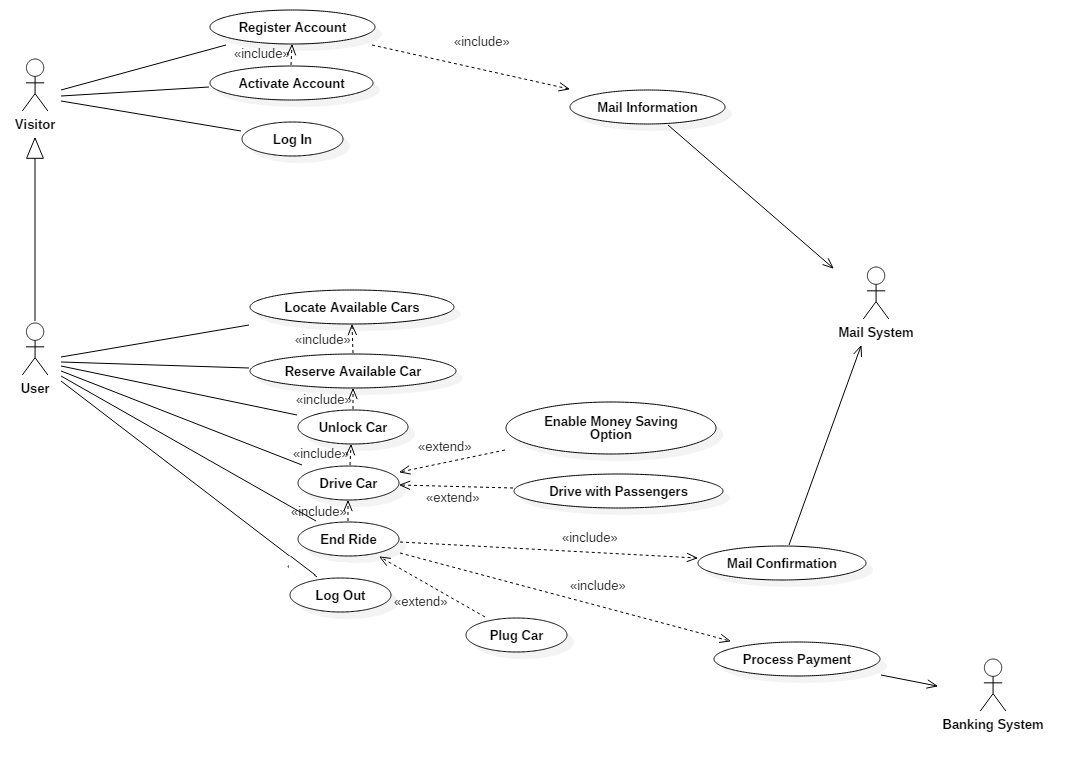
\includegraphics[width=\linewidth,keepaspectratio]{../Diagrams/UC/Use_Case.png}
\caption{Use Case}
\end{figure}
\FloatBarrier
\clearpage

\subsubsection{Activity Diagrams}
\begin{figure}[h]
\centering
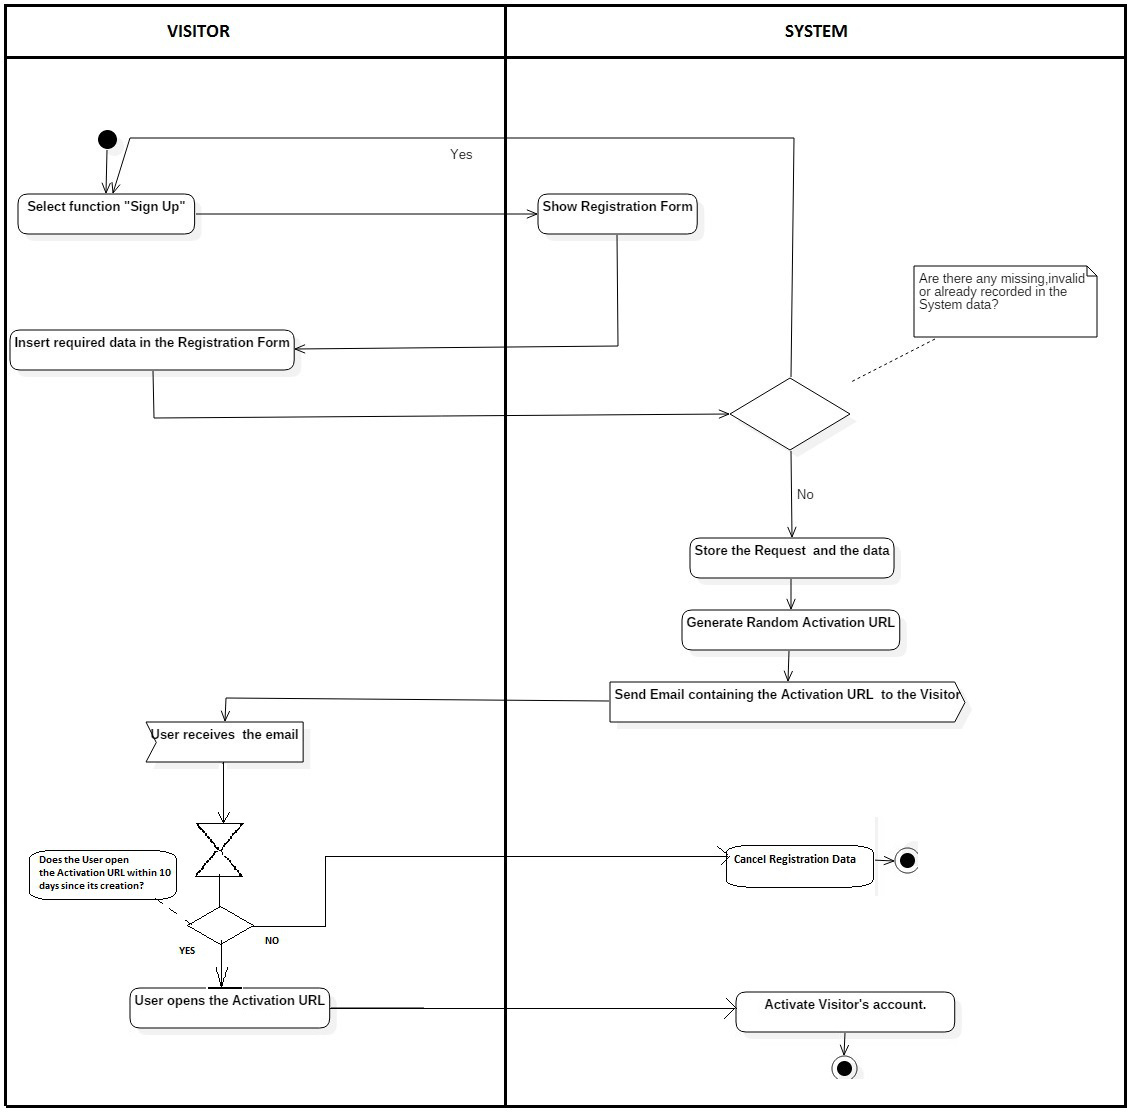
\includegraphics[width=\linewidth,keepaspectratio]{../Diagrams/AD/Registration.jpg}
\caption{Registration flowchart}
\end{figure}
\FloatBarrier
\begin{figure}[h]
\centering
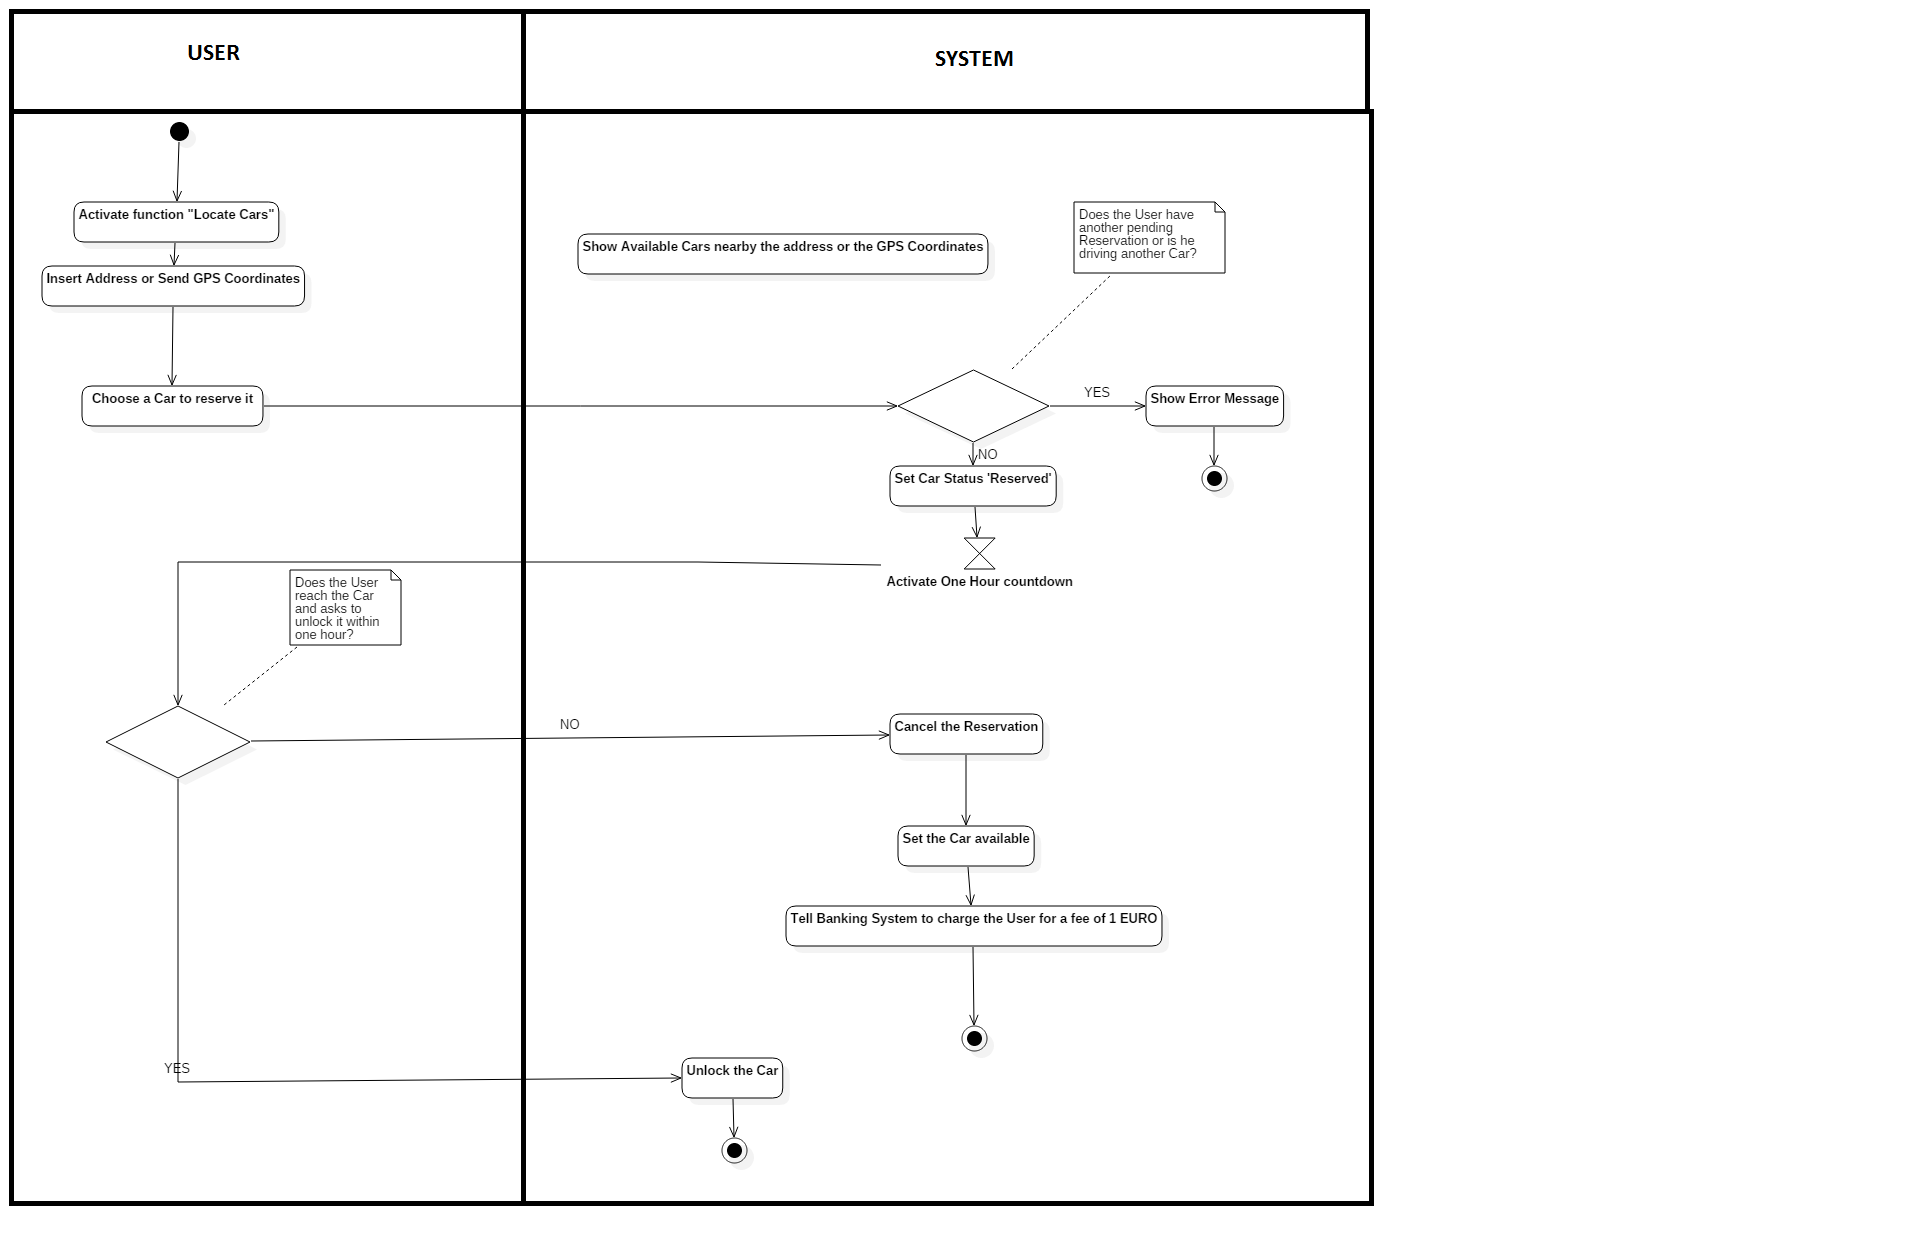
\includegraphics[width=\linewidth,keepaspectratio]{../Diagrams/AD/Locate_Reserve_Unlock.png}
\caption{Reservation flowchart}
\end{figure}
\FloatBarrier
\begin{figure}[h]
\centering
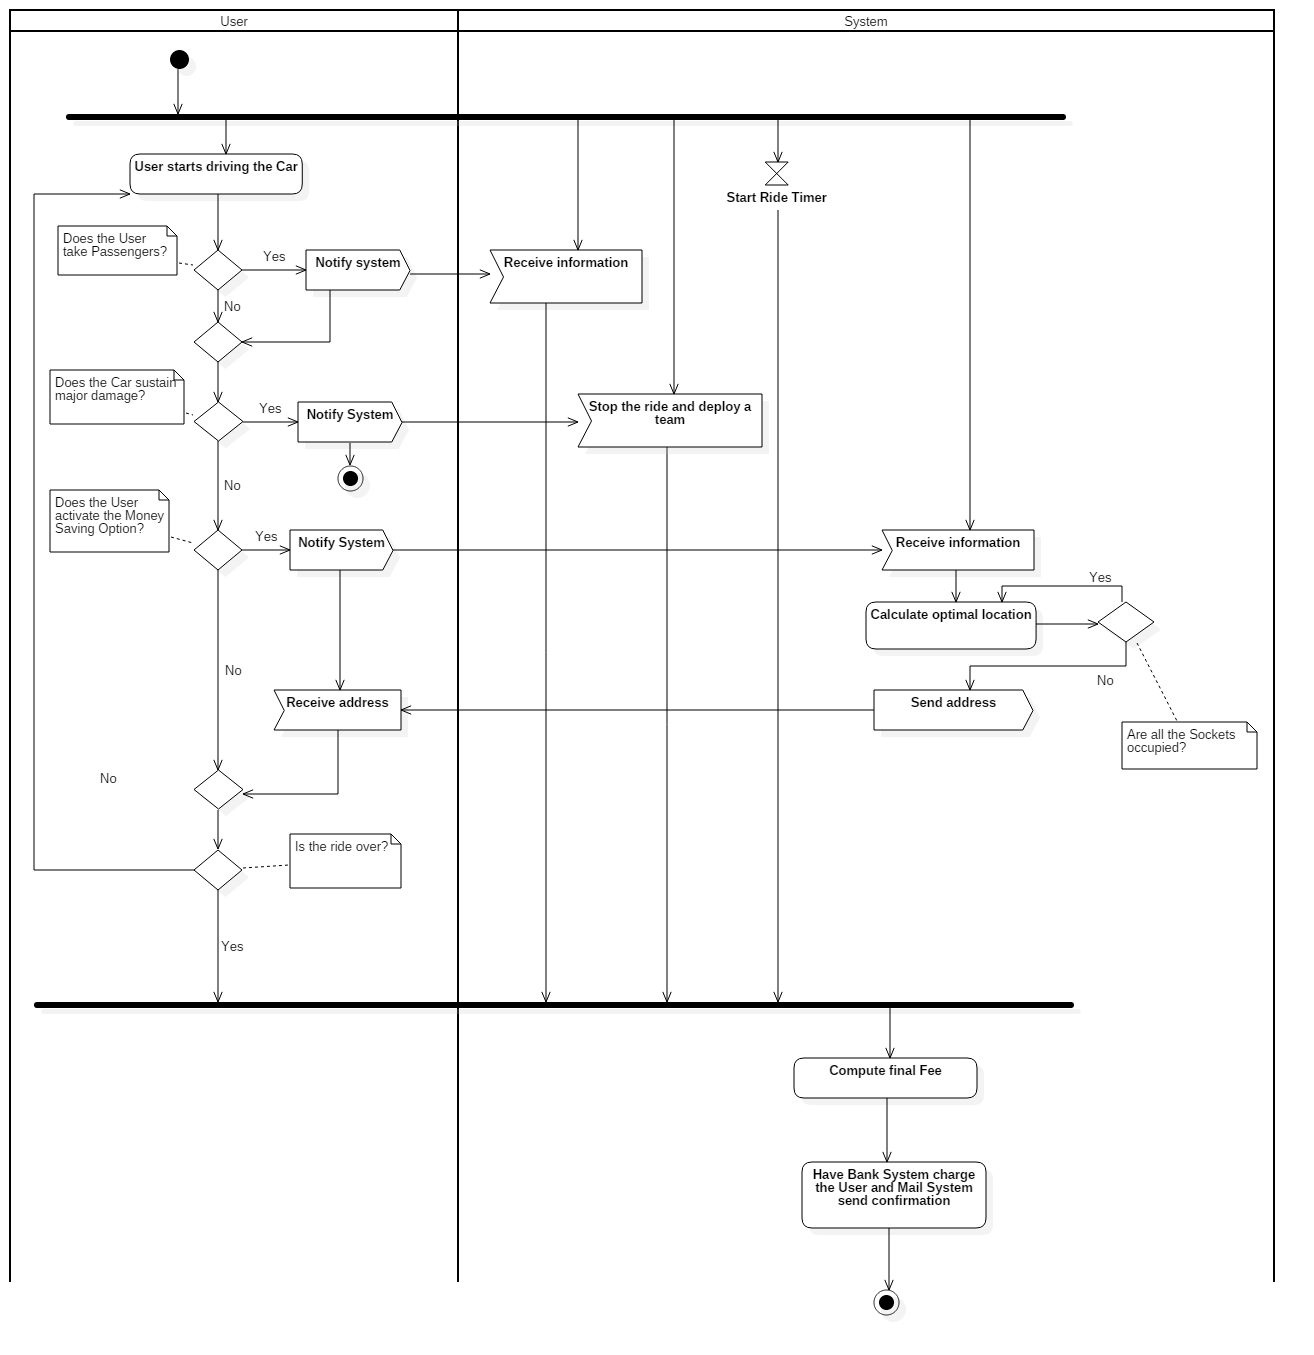
\includegraphics[width=\linewidth,keepaspectratio]{../Diagrams/AD/Ride.png}
\caption{Ride flowchart}
\end{figure}
\FloatBarrier

\subsubsection{Sequence Diagrams}
\begin{figure}[h]
\centering
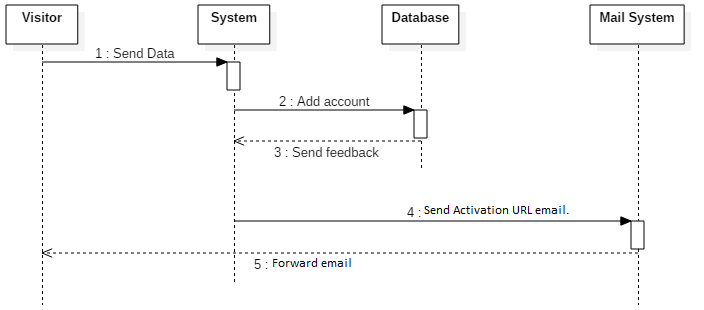
\includegraphics[width=\linewidth,keepaspectratio]{../Diagrams/SD/UC_1.png}
\caption{Use Case 1}
\end{figure}
\FloatBarrier
\begin{figure}[h]
\centering
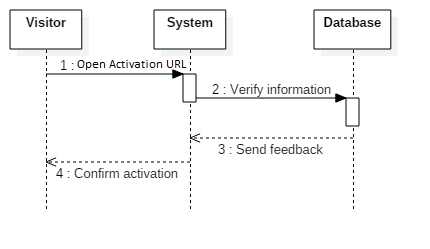
\includegraphics[width=\linewidth,keepaspectratio]{../Diagrams/SD/UC_2.png}
\caption{Use Case 2}
\end{figure}
\FloatBarrier
\begin{figure}[h]
\centering
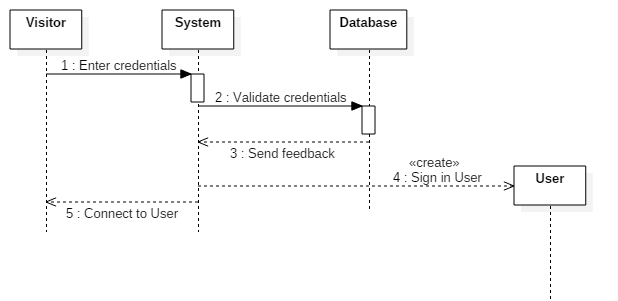
\includegraphics[width=\linewidth,keepaspectratio]{../Diagrams/SD/UC_3.png}
\caption{Use Case 3}
\end{figure}
\FloatBarrier
\begin{figure}[h]
\centering
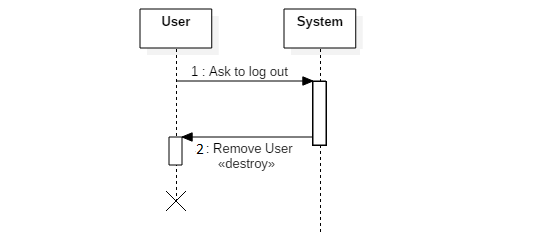
\includegraphics[width=\linewidth,keepaspectratio]{../Diagrams/SD/UC_4.png}
\caption{Use Case 4}
\end{figure}
\FloatBarrier
\begin{figure}[h]
\centering
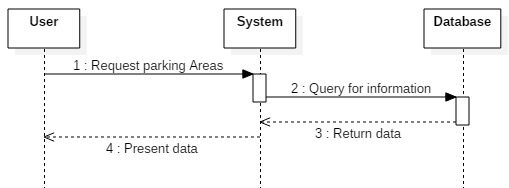
\includegraphics[width=\linewidth,keepaspectratio]{../Diagrams/SD/UC_5.png}
\caption{Use Case 5}
\end{figure}
\FloatBarrier
\begin{figure}[h]
\centering
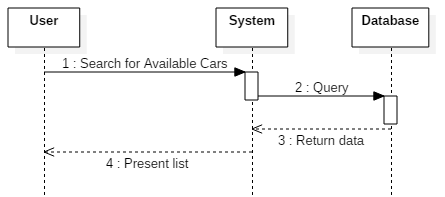
\includegraphics[width=\linewidth,keepaspectratio]{../Diagrams/SD/UC_6.png}
\caption{Use Case 6}
\end{figure}
\FloatBarrier
\begin{figure}[h]
\centering
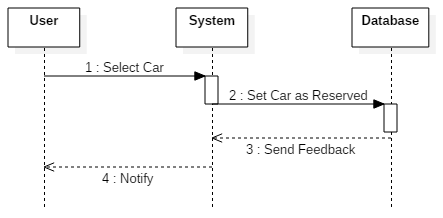
\includegraphics[width=\linewidth,keepaspectratio]{../Diagrams/SD/UC_7.png}
\caption{Use Case 7}
\end{figure}
\FloatBarrier
\begin{figure}[h]
\centering
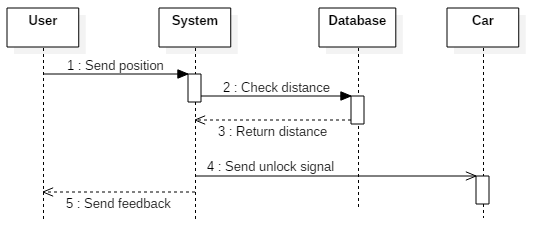
\includegraphics[width=\linewidth,keepaspectratio]{../Diagrams/SD/UC_8.png}
\caption{Use Case 8}
\end{figure}
\FloatBarrier
\begin{figure}[h]
\centering
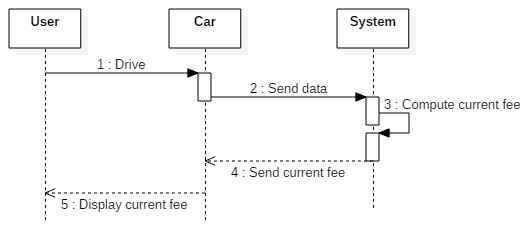
\includegraphics[width=\linewidth,keepaspectratio]{../Diagrams/SD/UC_9.png}
\caption{Use Case 9}
\end{figure}
\FloatBarrier
\begin{figure}[h]
\centering
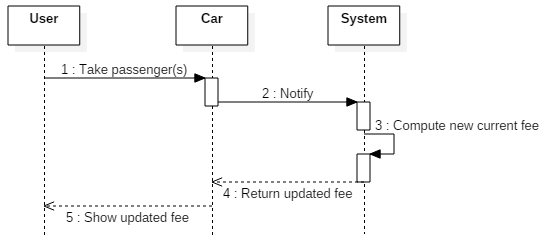
\includegraphics[width=\linewidth,keepaspectratio]{../Diagrams/SD/UC_10.png}
\caption{Use Case 10}
\end{figure}
\FloatBarrier
\begin{figure}[h]
\centering
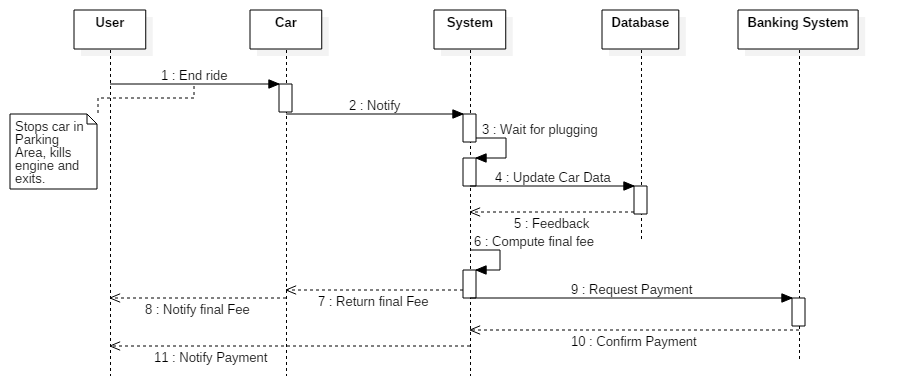
\includegraphics[width=\linewidth,keepaspectratio]{../Diagrams/SD/UC_11.png}
\caption{Use Case 11}
\end{figure}
\FloatBarrier
\begin{figure}[h]
\centering
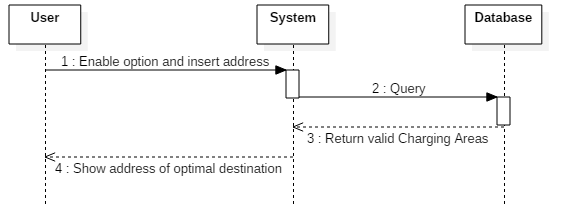
\includegraphics[width=\linewidth,keepaspectratio]{../Diagrams/SD/UC_12.png}
\caption{Use Case 12}
\end{figure}
\FloatBarrier

\clearpage
\subsubsection{Class Diagram}
\begin{figure}[h]
\centering
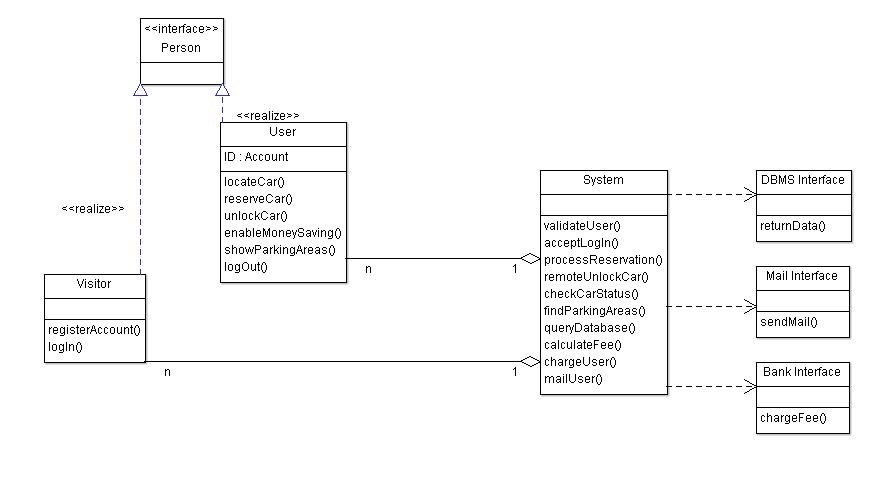
\includegraphics[width=\linewidth,keepaspectratio]{../Diagrams/CD/Class_Diagram.png}
\caption{Class Diagram}
\end{figure}
\FloatBarrier

\clearpage
\subsubsection{Statechart Diagram}
\begin{figure}[h]
\centering
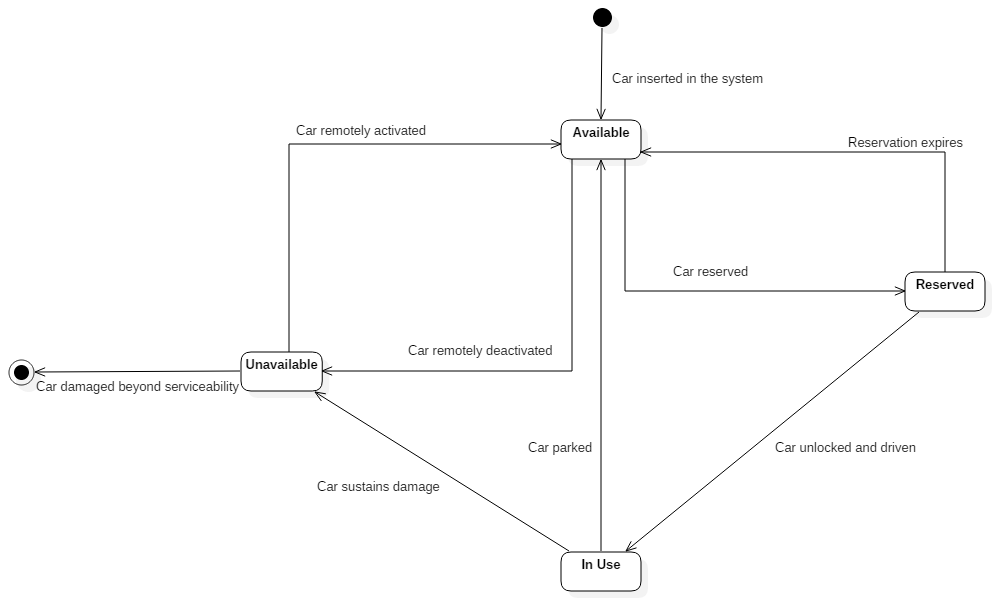
\includegraphics[width=\linewidth,keepaspectratio]{../Diagrams/SCD/SCD_Car.png}
\caption{Statechart diagram of Car}
\end{figure}
\FloatBarrier

\subsubsection{Traceability Matrix}
%TODO Traceability Matrix
\newcounter{idcounter}
\begin{center}
  \begin{longtable}{|p{.15\textwidth}|p{.12\textwidth}|p{.26\textwidth}|p{.23\textwidth}|p{.26\textwidth}|}
    \hline
    \stepcounter{idcounter}
    \textbf{Raw ID} & \textbf{Goal ID} & \textbf{Requirement ID} & \textbf{Use Case ID}   \\ \hline   
    \theidcounter & G1 & R1 & UC1 \\ \hline
    \stepcounter{idcounter}
    \theidcounter & G1 & R1 & UC2 \\ \hline
    \stepcounter{idcounter}
    \theidcounter & G2 & R1 & UC3 \\ \hline
    \stepcounter{idcounter}
    \theidcounter& G3 &  R2 & UC6\\ \hline
    \stepcounter{idcounter}
    \theidcounter & G4 & & UC7\\ \hline
    \stepcounter{idcounter}
    \theidcounter & G5 & & UC8\\ \hline
    \stepcounter{idcounter}
    \theidcounter & G6 & & UC8\\ \hline
    \stepcounter{idcounter}
    \theidcounter & G7 & & UC9\\ \hline
    \stepcounter{idcounter}
    \theidcounter & G8 & & UC9\\ \hline
    \stepcounter{idcounter}
    \theidcounter & G9 & & UC5\\ \hline   
    \stepcounter{idcounter}
    \theidcounter & G10 & & UC11\\ \hline
    \stepcounter{idcounter}
    \theidcounter & G11 & & U10\\ \hline
    \stepcounter{idcounter}
    \theidcounter & G11 & & UC11\\ \hline
    \stepcounter{idcounter}
    \theidcounter & G12 & & UC11\\ \hline    
    \stepcounter{idcounter}
    \theidcounter & G13 & & UC11\\ \hline   
     \stepcounter{idcounter}
    \theidcounter & G13 & & UC12\\ \hline    
    \stepcounter{idcounter}
    \theidcounter & G14 & & UC11\\ \hline    
    \stepcounter{idcounter}
    \theidcounter & G15 & & UC13\\ \hline
  \end{longtable}
\end{center}


\subsection{Non-Functional Requirements}
Our stakeholders did not force any special requirements

Additional requirements that may be added to improve on the program.
\subsubsection{Performance Requirements}
\subsubsection{Safety and Security Requirements}
\subsubsection{Software Quality Attributes}
\subsubsection{Availability}
\subsubsection{Reliability}
\subsubsection{Extensibility}
\subsubsection{Interoperability}
\subsubsection{Business Rules}
\subsection{External Interface Requirements}
The interfaces the system should interact with.

\subsubsection{Software Interface}
\subsubsection{Hardware Interface}
The central server must be provided with one or more sufficiently advanced computers that may run the server-side application, and allow it access to a high-speed network connection.

The client application must be developed so as to have access to both the phone's network connection and its GPS locator.

\subsubsection{User Interface}
The User Interface is provided by the client smartphone application, and allows the user to perform all of their actions.

\subsubsection{Communication Interface}
As mentioned above, the System heavily uses Internet communications protocols, mainly the HTTP protocol. HTTP requests to and from the server will be mostly carried by mobile network connections.

\subsection{Performance Requirements}
\subsection{Design Constraints}
\subsection{Software System Attributes}
The System does not need to interface with external software. Database management can be performed via the Administrative Access function.

\subsection{Other Requirements}

%Maybe
\clearpage\section{Appendix}
\end{document}